%%%%% Technical Details %%%%%

\chapter{Installing and Using ``Processing Abstractions''} \label{app_setup}

In order to set up Processing Abstractions, first download \ac{GT} from \url{https://gtoolkit.com/download/} for your platform and extract the archive's entire content.

Before running it, create a new text file called \ct{startup.st} in \ac{GT}'s top-level folder besides \ct{GlamorousToolkit.image} with the following content (access it through figure \ref{fig_startup_st_qr}):

\begin{code}
Metacello new
	repository: 'github://zeniko/\ac{GT}-exploration:thesis/src';
	baseline: 'GtExploration';
	load.
Metacello new
	repository: 'github://zeniko/processing-abstractions:thesis/src';
	baseline: 'ProcessingAbstractions';
	load.

"Hide the 'Implementation and Tests' section."
GtExplorationHomeSection studentMode: true.

"Make indenting keyboard shortcuts available to non-US-English keyboard layouts
(cf. https://github.com/feenkcom/gtoolkit/issues/3002)."
LeSnippetElement keyboardShortcuts
	at: #IndentSnippet
		put: BlKeyCombinationBuilder new alt shift arrowRight build;
	at: #UnindentSnippet
		put: BlKeyCombinationBuilder new alt shift arrowLeft build.

"Make the zoom in keyboard shortcut available to de-CH keyboard layouts
(cf. https://github.com/feenkcom/gtoolkit/issues/4624)."
TLeWithFontSize compile:
	((TLeWithFontSize methodNamed: #initializeFontSizeShortcuts) sourceCode
		copyReplaceAll: 'equal' with: 'shift minus').

"Patch unneeded addressbar out of YouTube snippet
(cf. https://github.com/feenkcom/gtoolkit/issues/4560)."
LeYoutubeReferenceElement compile:
	((LeYoutubeReferenceElement methodNamed: #updatePicture) sourceCode
		copyReplaceAll: '</iframe>'' ' with: '</iframe>''; removeChildAt: 1 ').
\end{code}

Finally, run the \ct{GlamorousToolkit} executable (under Windows and Linux it is located in the \ct{bin} subfolder). The teaching materials of Processing Abstractions are now available behind the ``Unterrichtseinheiten'' home tile.

Verify that everything works as desired, and then close and save the changes to the image.

\emph{Warning:} If you have already used \ac{GT} before, the contents of your local knowledge database will also be included in \ac{GT}'s image. Therefore, rename that folder (usually \ct{lepiter/default} in your documents folder) before starting the \ac{GT} meant for distribution, and undo the renaming before starting your own \ac{GT} instance again.

Also, since the executable \ct{GlamorousToolkit.exe} is located in a subdirectory under Windows and Linux, adding a top-level link can help students. See \url{https://github.com/zeniko/gtRunner} for a ready-to-use drop-in.

\begin{cfigure}[fig_startup_st_qr]{QR-link to the code for \ct{startup.st} for convenience}
\href{https://github.com/zeniko/gyminf-thesis/blob/main/appendix.tex}{
\includegraphics[height=2.5cm]{startup.st}}
\end{cfigure}



\chapter{GT Processing API} \label{app_api}

This appendix lists the available \ac{API} calls implemented in Processing Abstraction's partial implementation of Processing.\footnote{For comparison, the full \ac{API} or Processing's Python mode is available at \archivedurl{https://py.processing.org/reference/}.} This has been autogenerated from the \ac{GT} page ``Processing API'':

\section{Rendering}

\subsection{Setup}
\begin{description}
\item[\texttt{background(r, g, b)}] \hfill \\
	Clears the canvas and changes its color (see \ct{fill(r, g, b)}). Default is light gray (192, 192, 192).
\item[\texttt{background(gray)}] \hfill \\
	Clears the canvas and changes its color (see \ct{fill(gray)}). Default is light gray (192).
\item[\texttt{size(width, height)}] \hfill \\
	Prepares an output canvas of the given dimensions. This command must always be called first (for animations: first command in \ct{def setup}).
\end{description}

\subsection{Shapes}
\begin{description}
\item[\texttt{ellipse(x, y, dx, dy)}] \hfill \\
	Draws an ellipse with the given diameters and its center at \ct{(x; y)}.
\item[\texttt{image(image, x, y)}, \texttt{image(image, x, y, width, height)}] \hfill \\
	Renders the image loaded with \ct{loadImage(...)} at the given coordinates (and scales it to fit the given size). Arguments following after the first are identical to \ct{rect}'s. If \ct{width} and \ct{height} are not given, the image's native dimensions are used.
\item[\texttt{line(x1, y1, x2, y2)}] \hfill \\
	Draws a line from \ct{(x1; y1)} to \ct{(x2; y2)}.
\item[\texttt{loadImage(pathOrUrl)}] \hfill \\
	Loads the image from the given URL or path. The returned value is to be used with \ct{image(...)}.
Paths can be absolute or relative to either \ct{FileLocator class>>gtResource} or:
\begin{code}
Element
GtInspector newOn: FileLocator documents / 'lepiter'
\end{code}
\item[\texttt{rect(x, y, width, height)}] \hfill \\
	Draws a rectangle of the given width and height, parallel to the coordinate axes with its top left corner at \ct{(x; y)}. If an optional fifth argument is given, corners are rounded by that many pixels.
\item[\texttt{text(string, x, y)}] \hfill \\
	Renders the given \ct{string} with its baseline starting at \ct{(x; y)}.
\item[\texttt{textSize(size)}] \hfill \\
	Sets the size for rendering text in pixels. Default is 12px.
\item[\texttt{triangle(x1, y1, x2, y2, x3, y3)}] \hfill \\
	Draws a triangle with its vertices at the points \ct{(x1; y1)}, \ct{(x2; y2)} and \ct{(x3; y3)}.
\end{description}

\subsection{Colors}
\begin{description}
\item[\texttt{color(r, g, b)}, \texttt{color(gray)}] \hfill \\
	Generates a color object which can be stored in a variable also be used with \ct{fill(...)}, \ct{stroke(...)} and \ct{background(...)}.
\item[\texttt{fill(r, g, b)}] \hfill \\
	Selects the color to use for filling rendered shapes. The color is given as three values in the range of 0 to 255 (red, green and blue respectively). Default is white (255, 255, 255).
\item[\texttt{fill(gray)}] \hfill \\
	Selects the gray scale value to use for filling rendered shapes. The color is given as a single value in the range of 0 to 255 (black/dark to white/light). Default is white (255).
\item[\texttt{noStroke()}] \hfill \\
	Disables borders for future shapes. Equivalent to \ct{strokeWeight(0)}.
\item[\texttt{stroke(r, g, b)}] \hfill \\
	Selects the color to use for the borders of rendered shapes (see \ct{fill(r, g, b)}). Default is black (0, 0, 0).
\item[\texttt{stroke(gray)}] \hfill \\
	Selects the gray scale value to use for the borders of rendered shapes (see \ct{fill(gray)}). Default is black (0).
\item[\texttt{strokeWeight(weight)}] \hfill \\
	Determines the size of drawn borders in pixels. Default is 0.5px.
\end{description}

\subsection{Transforms}
\begin{description}
\item[\texttt{rotate(angle)}] \hfill \\
	Rotates all future shapes by the given angle (in \ct{radians}!) clockwise around the origin.
\item[\texttt{scale(factor)}] \hfill \\
	Linearly scales all future shapes by the given factor from the origin.
\item[\texttt{translate(x, y)}] \hfill \\
	Moves the origin \ct{(0; 0)} for all future shapes (defaults to the upper left corner).
\end{description}

\section{Events}
\begin{description}
\item[\texttt{def draw():}] \hfill \\
	is called repeatedly (up to \ct{frameRate} times per second) for drawing the output.
\item[\texttt{def mouseClicked():}] \hfill \\
	is called whenever a mouse button has been clicked \emph{and} released.
\item[\texttt{def mouseMoved():}] \hfill \\
	is called whenever the mouse has been moved. Alternatively query \ct{mouseX} and \ct{mouseY} in \ct{draw()}.
\item[\texttt{def mousePressed():}] \hfill \\
	is called whenever a mouse button has been pressed. Alternatively query \ct{mousePressed} in \ct{draw()}.
\item[\texttt{def mouseReleased():}] \hfill \\
	is called whenever a mouse button has been released.
\item[\texttt{def setup():}] \hfill \\
	is called once as the program starts.
\end{description}

\section{Mathematics}
\begin{description}
\item[\texttt{cos(angle)}] \hfill \\
	Returns the cosine value for the given angle (measured in radians).
\item[\texttt{int(value)}] \hfill \\
	Rounds the value to an integer.
\item[\texttt{PI}] \hfill \\
	The value of the mathematical constant p.
\item[\texttt{max(a, b)}] \hfill \\
	Returns the larger of the two values (\ct{max(a)} returns the largest value contained in the list \ct{a}).
\item[\texttt{min(a, b)}] \hfill \\
	Returns the smaller of the two values (\ct{min(a)} returns the smallest value contained in the list \ct{a}).
\item[\texttt{radians(angle)}] \hfill \\
	Converts the given angle (measured in degrees) into radians.
\item[\texttt{random(limit)}] \hfill \\
	Returns a random floating point number between 0 and limit (inclusive).
\item[\texttt{randomSeed(seed)}] \hfill \\
	Reinitializes the random generator with the given \ct{seed} number. Using the same number will result in the exact same sequence of pseudo-randomly generated numbers.
\item[\texttt{sin(angle)}] \hfill \\
	Returns the sine value for the given angle (measured in radians).
\item[\texttt{sqrt(value)}] \hfill \\
	Returns the square root of the given value.
\item[\texttt{tan(angle)}] \hfill \\
	Returns the tangent value for the given angle (measured in radians).
\end{description}

\section{Lists}
Lists are objects which provide their own methods. Note that for the following commands, \ct{list} is a variable referencing a \ct{list}.
\begin{description}
\item[\texttt{len(list)}] \hfill \\
	Returns the number of items in this list.
\item[\texttt{list.append(value)}] \hfill \\
	Appends the value to the end of the list.
(\ct{list + [value]} instead produces a \emph{new} list. \ct{list + otherList} produces a \emph{new} list out of two lists.)
\item[\texttt{list.pop()}] \hfill \\
	Removes the last item from the list and returns the removed argument.
(\ct{list[:-1]} instead produces a \emph{new} list without the last item.)
\item[\texttt{list.reverse()}] \hfill \\
	Reverses this list's items.
(\ct{list[::-1]} instead produces a \emph{new} list with its items reversed.)
\item[\texttt{list.sort()}] \hfill \\
	Sorts this list's items.
(\ct{sorted(list)} instead produces a \emph{new} sorted list.)
\end{description}

\section{Miscellanea}
\begin{description}
\item[\texttt{delay(ms)}] \hfill \\
	Waits \ct{ms} milliseconds before continuing (mainly needed for demonstration purposes).
\item[\texttt{frameRate(fps)}] \hfill \\
	Limits the frame rate of animations to a maximum of \ct{fps} frames per second. Default is 30.
\item[\texttt{height}] \hfill \\
	Contains the canvas height as set by \ct{size()}.
\item[\texttt{millis()}] \hfill \\
	Returns the number of milliseconds that have passed since the program has started.
\item[\texttt{mouseX}, \texttt{mouseY}, \texttt{mousePressed}] \hfill \\
	Contains the \ct{x}- and \ct{y}-coordinates of the mouse cursor and whether the mouse has been pressed at the start of a \ct{draw}-phase (undefined outside of \ct{draw}).
\item[\texttt{print(value)}, \texttt{println(value)}] \hfill \\
	Prints the given value into an output console (mainly for debugging and for graphic-less program).
\item[\texttt{str(value)}] \hfill \\
	Turns the value into a string, e.\,g. for concatenating several values for use with \ct{text(...)}.
\item[\texttt{width}] \hfill \\
	Contains the canvas width as set by \ct{size()}.
\end{description}




\chapter{Technical Implementation of ``Processing Abstractions''} \label{app_implementation}


\section{Classes}


\begin{cfigure}[fig_uml_snippet]{Diagram of classes involved in \ct{LeProcessingSnippet}}
\begin{tikzpicture}

\begin{package}{Snippet}

\begin{class}[text width=6.6cm]{LeProcessingSnippet}{0, 0}
\end{class}

\begin{class}[text width=6.6cm]{LeProcessingSnippetViewModel}{0, 2}
\end{class}

\begin{class}[text width=6.6cm]{LeProcessingSnippetElement}{0, 4}
\end{class}

\begin{class}[text width=6.6cm]{GtProcessingCoderModel}{8, 0}
\end{class}

\begin{class}[text width=6.6cm]{GtProcessingCoderViewModel}{8, 4}
\operation{doIt:}
\operation{doItAndGo:}
\operation{doItAndGoAsynchronous:}
\operation{doItAndGoSerialized:}
\operation{doItAndPublish:with:}
\end{class}

\draw[umlcd style dashed line, ->] (LeProcessingSnippet) -- node[black]{asSnippetViewModel} (LeProcessingSnippetViewModel);
\draw[umlcd style dashed line, ->] (LeProcessingSnippetViewModel) -- node[black]{snippetElementClass} (LeProcessingSnippetElement);
\draw[umlcd style dashed line, ->] (LeProcessingSnippet) -- node[black, rotate=90]{newCoder} (GtProcessingCoderModel);
\draw[umlcd style dashed line, ->] (GtProcessingCoderModel) -- node[black]{asCoderViewModel} (GtProcessingCoderViewModel);

\end{package}

\end{tikzpicture}

\end{cfigure}


\section{Views}

The following views are available as arguments for \ct{ProcessingSource>>>renderLiveView:} (see page \pageref{embedding_view}). See figure \ref{fig_uml_views} for an overview of all view implementors.

\begin{cfigure}[fig_uml_views]{Diagram of all views provided and their implementors (methods set in \textit{italics} are forwarded)}
\begin{tikzpicture}

\begin{package}{Processing}

\begin{class}[text width=6cm]{ProcessingSource}{8, 0}
\operation[0]{gtAbstractionsFor:}
\operation[0]{gtBytecodeFor:}
\operation[0]{gtIntermediaryRepresentationFor:}
\operation[0]{gtOutputFor:}
\operation[0]{gtSourceCodeFor:}
\operation[0]{gtTranspilationFor:}
\operation[0]{gtTreeFor:}
\end{class}

\begin{class}[text width=7cm]{ProcessingProgram}{0, 9.5}
\operation{gtAbstractionsFor:}
\operation[0]{gtBytecodeFor:}
\operation{gtBytecodePlusIRFor:}
\operation{gtBytecodePlusSourceFor:}
\operation[0]{gtHexDumpFor:}
\operation[0]{gtIntermediaryRepresentationFor:}
\operation{gtIntermediaryRepresentationPlusSourceFor:}
\operation[0]{gtOutputFor:}
\operation{gtOutputPlusSourceFor:}
\operation[0]{gtOutputShapesFor:}
\operation[0]{gtSlicesFor:}
\operation{gtSourceBytesFor:}
\operation{gtSourceBytesPlusCharsFor:}
\operation{gtSourceBytesPlusSourceFor:}
\operation{gtSourceCharsFor:}
\operation{gtSourceCharsPlusSourceFor:}
\operation{gtSourceCodeFor:}
\operation{gtStepsFor:}
\operation{gtTokensFor:}
\operation{gtTokensPlusSourceFor:}
\operation{gtTokensPlusTreeFor:}
\operation[0]{gtTranspilationFor:}
\operation{gtTranspilationPlusSourceFor:}
\operation{gtTranspilationPostfixFor:}
\operation{gtTranspilationPrefixFor:}
\operation{gtTreeFor:}
\operation{gtTreeMondrianFor:}
\operation{gtTreePlusSourceFor:}
\end{class}

\begin{interface}[text width=6cm]{ProcessingCodeBase}{8, 4.5}
\operation{gtAbstractionsFor:}
\operation{gtBytecodeFor:}
\operation{gtHexDumpFor:}
\operation{gtIntermediaryRepresentationFor:}
\operation{gtOutputFor:}
\operation{gtSlicesFor:}
\operation{gtTranspilationFor:}
\end{interface}

\begin{class}[text width=6cm]{ProcessingCanvas}{8, 7.5}
\operation{asElement}
\operation{gtOutputFor:}
\operation{gtOutputShapesFor:}
\end{class}

\begin{class}[text width=6cm]{ProcessingRunStep}{8, 13}
\operation{gtAbstractionsFor:}
\operation{gtBytecodeFor:}
\operation{gtOutputFor:}
\operation{gtOverviewFor:}
\operation[0]{gtSourceCodeFor:}
\operation{gtStackFor:}
\operation[0]{gtTranspilationPlusSourceFor:}
\operation{gtVariablesFor:}
\end{class}

\begin{class}[text width=7cm]{ProcessingTranspilationSlice}{0, 13}
\operation{gtSourceCodeFor:}
\operation{gtTranspilationFor:}
\operation{gtTranspilationPlusSourceFor:}
\end{class}

\draw[umlcd style dashed line, ->] (ProcessingSource.south west) -| node[black]{$<<$forwards to$>>$} (ProcessingProgram.south);
\draw[umlcd style dashed line, ->] (ProcessingProgram.north east) -- +(0.5, 0) -- +(0.5, -9.1) -| node[black]{$<<$forwards to$>>$} (ProcessingCodeBase.south);
\draw[umlcd style dashed line, ->] (ProcessingProgram.north east) -- +(0.5, 0) -- +(0.5, -1.5) -| node[black]{$<<$forwards to$>>$} (ProcessingCanvas);
\draw[umlcd style dashed line, ->] (ProcessingCodeBase) -- node[black]{$<<$embeds$>>$} (ProcessingCanvas);
\draw[umlcd style dashed line, ->] (ProcessingProgram.north east) -- +(0.5, 0) -- +(0.5, -1) -| node[black]{$<<$embeds$>>$} (ProcessingRunStep);
\draw[umlcd style dashed line, ->] (ProcessingRunStep.west) -- +(-0.5, 0) -- +(-0.5, -0.5) -| node[black]{$<<$forwards to$>>$} (ProcessingTranspilationSlice);

\end{package}

\end{tikzpicture}

\end{cfigure}

\begin{description}
\item[\texttt{gtAbstractionsFor:}] \hfill \\
	(implemented by \ct{ProcessingProgram}) combines \ct{gtSourceCodeFor:}, \ct{gtTreeFor:}, \ct{gtBytecodeFor:}, and \ct{gtOutputFor:}, linking the source to the other three views through a common \ct{Announcer} reacting to selection changes (shown in figure \ref{fig_view_abstractions}).
\item[\texttt{gtBytecodeFor:}] \hfill \\
	uses the \ct{CompiledMethod} instances of each method in a compiled class' \ct{class methodDict} to access its \ct{symbolicBytecodes} and show the resulting \ct{SymbolicBytecode}s' bytes and mnemonic (shown on the right in figure \ref{fig_view_ir_bytecode}). \ct{gtBytecodePlusSourceFor:} combines this view with \ct{gtSourceCodeFor:}.
\item[\texttt{gtBytecodePlusIRFor:}] \hfill \\
	combines the \ct{gtBytecodeFor:} with \ct{gtIntermediaryRepresentationFor:} (shown in figure \ref{fig_view_ir_bytecode}).
\item[\texttt{gtHexDumpFor:}] \hfill \\
	shows individual bytes for all compiled methods.
\item[\texttt{gtIntermediaryRepresentationFor:}] \hfill \\
	uses the \ct{OpalCompiler} to translate the transpiled Smalltalk code to \ct{IRInstruction}s (shown on the left in figure \ref{fig_view_ir_bytecode}). \ct{gtIntermediaryRepresentationPlusSourceFor:} combines this view with \ct{gtSourceCodeFor:}.
\item[\texttt{gtOutputFor:}] \hfill \\
	displays a newly created \ct{ProcessingCanvasElement} with attached event listeners for interactivity (shown on the bottom right in figure \ref{fig_view_abstractions}). \ct{gtOutputPlusSourceFor:} combines this view with \ct{gtSourceCodeFor:}.
\item[\texttt{gtOutputShapesFor:}] \hfill \\
	shows a list of all \ct{ProcessingCanvasShape}s in the order they were drawn (shown in figure \ref{fig_view_shapes}). Clearing the canvas with \ct{background(...)} also clears this list.
\item[\texttt{gtSlicesFor:}] \hfill \\
	shows a list of \ct{ProcessingTranspilationSlice}s with the corresponding expressions in Processing source code and Smalltalk transpilation highlighted (shown in figure \ref{fig_view_slices}).
\item[\texttt{gtSourceBytesFor:}] \hfill \\
	shows a list of \ct{SmallInteger}s corresponding to the bytes of the source code after UTF-8 encoding (shown on the right in figure \ref{fig_view_chars_bytes}) \ct{gtSourceBytesPlusSourceFor:} combines this view with \ct{gtSourceCodeFor:}.
\item[\texttt{gtSourceBytesPlusCharsFor:}] \hfill \\
	combines \ct{gtSourceCharsFor:} and \ct{gtSourceBytesFor:} (shown in figure \ref{fig_view_chars_bytes}).
\item[\texttt{gtSourceCharsFor:}] \hfill \\
	shows a list of \ct{Character}s corresponding to each of the Processing source code's characters (shown on the left in figure \ref{fig_view_chars_bytes}). \ct{gtSourceCharsPlusSourceFor:} combines this view with \ct{gtSourceCodeFor:}.
\item[\texttt{gtSourceCodeFor:}] \hfill \\
	displays a fresh read-only editor instance from \ct{SmaCCParseNode>>gtSourceEditorWithHightlight:} with a custom \ct{BrTextEditorReadonlyWithNavigationMode} mode (shown on the top left in figure \ref{fig_view_abstractions}, on the left in \ref{fig_view_transpilation}, \etc).
\item[\texttt{gtStepsFor:}] \hfill \\
	shows a list of \ct{ProcessingRunStep}s and their own \ct{gtAbstractionFor:} view, consisting of their \ct{gtSourceCodeFor:}, \ct{gtBytecodeFor:}, \ct{gtVariablesFor:}, \ct{gtStackFor:}, and \ct{gtOutputFor:} (shown in figure \ref{fig_view_runsteps}). \ct{ProcessingRunStep>>gtOverviewFor:} is a simplified variant of this shown from the Processing/Python snippet.
\item[\texttt{gtTokensFor:}] \hfill \\
	shows a list of \ct{SmaCCToken}s that were produced by \ct{ProcessingParser} (shown on the left in figure \ref{fig_view_tokens_ast}). \ct{gtTokensPlusSourceFor:} combines this view with \ct{gtSourceCodeFor:}.
\item[\texttt{gtTokensPlusTreeFor:}] \hfill \\
	combines \ct{gtTokensFor:} with \ct{gtTreeFor:} (shown in figure \ref{fig_view_tokens_ast}).
\item[\texttt{gtTranspilationFor:}] \hfill \\
	shows the transpiled Smalltalk code in \ct{GT}'s code viewer, which separates methods and adds syntax highlighting. \ct{gtTranspilationPlusSourceFor:} combines this view with \ct{gtSourceCodeFor:} (shown in figure \ref{fig_view_transpilation}).
\item[\texttt{gtTranspilationPostfixFor:} and \texttt{gtTranspilationPrefixFor:}] \hfill \\
	show a \ct{String} produced by \ct{ProcessingTranspilerVariant} in either its \ct{prefix} or \ct{postfix} modes (both shown at the bottom in figure \ref{fig_view_prefix_postfix}).
\item[\texttt{gtTreeFor:}] \hfill \\
	shows a treelist of \ct{PyRootNode}s for expression roots and \ct{SmaCCToken}s for structural tokens (shown on the right in figure \ref{fig_view_tokens_ast}).
\item[\texttt{gtTreeMondrianFor:}] \hfill \\
	shows a horizontal \ct{GtMondrian} tree produced by \ct{ProcessingTreeMondrianCreator} (shown in figure \ref{fig_view_ast_tree}). \ct{gtTreePlusSourceFor:} combines this view with \ct{gtSourceCodeFor:}.
\end{description}

\begin{cfigure}[fig_view_abstractions]{The Abstractions view with source code, \ac{AST}, bytecode, and output showing}
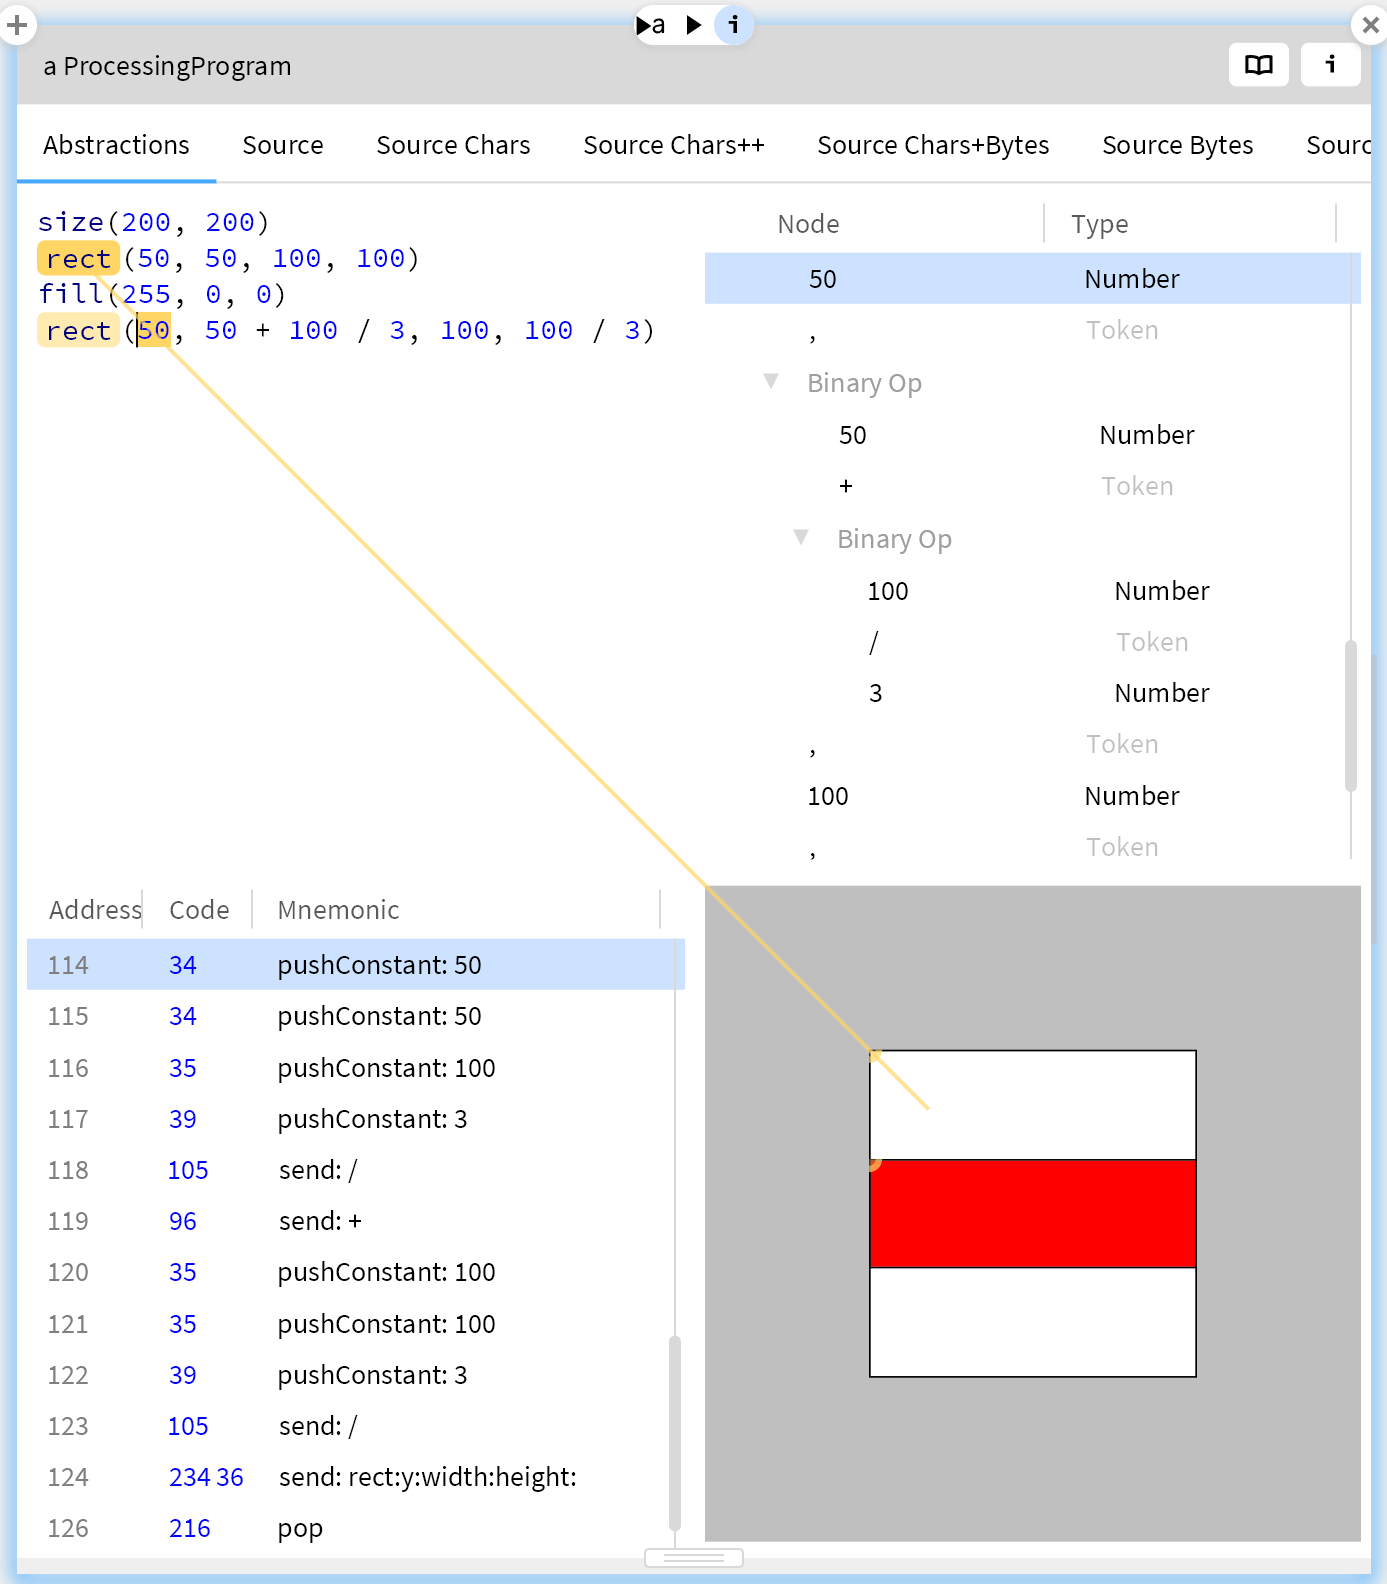
\includegraphics[width=.7\textwidth]{view_abstractions}
\end{cfigure}

\begin{cfigure}[fig_view_chars_bytes]{The Characters and Bytes views, connected}
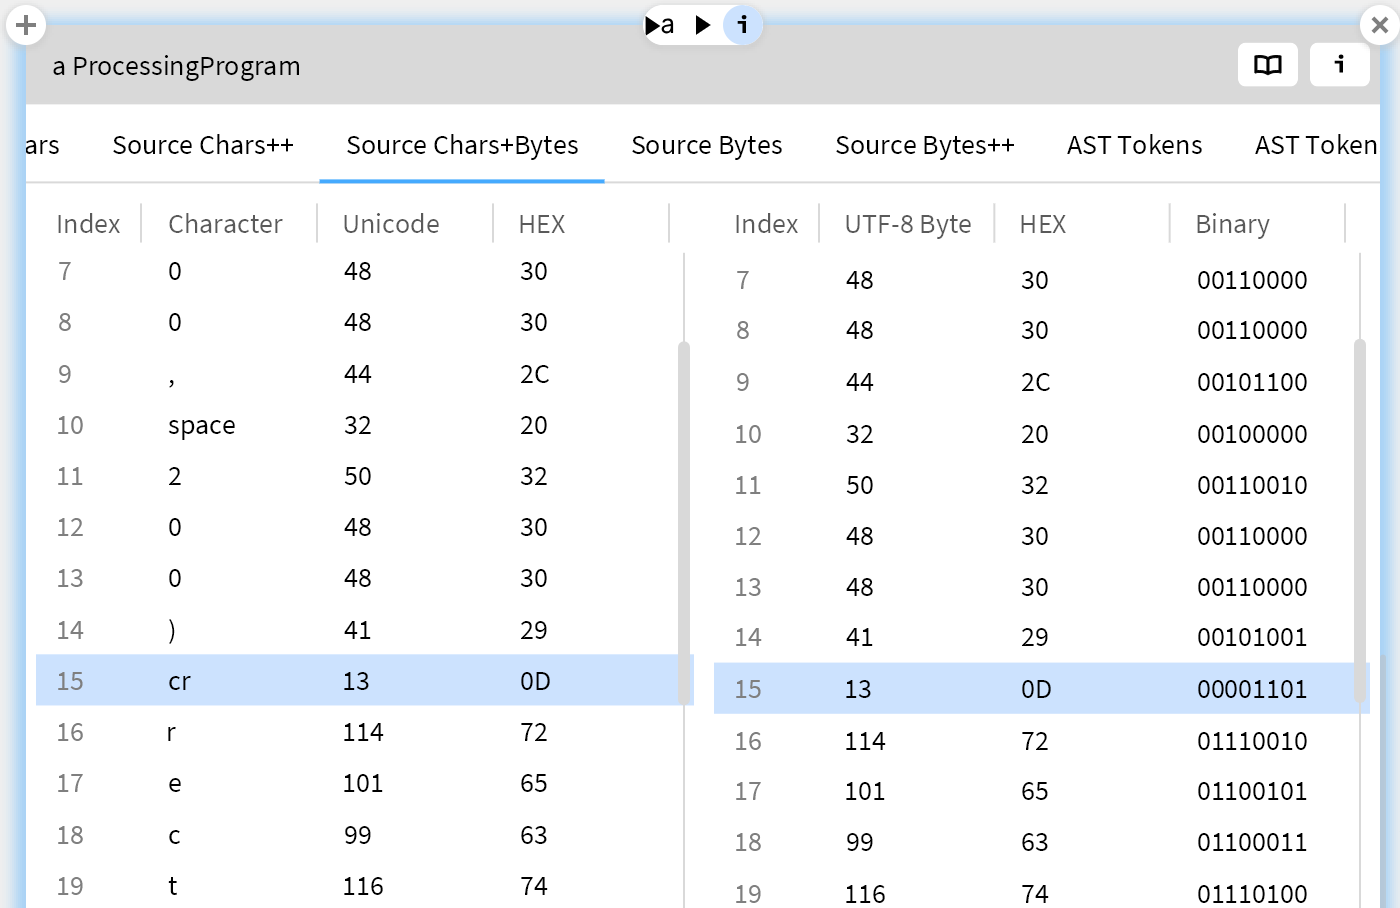
\includegraphics[width=.7\textwidth]{view_chars_bytes}
\end{cfigure}

\begin{cfigure}[fig_view_tokens_ast]{The Tokens and \ac{AST} views, connected}
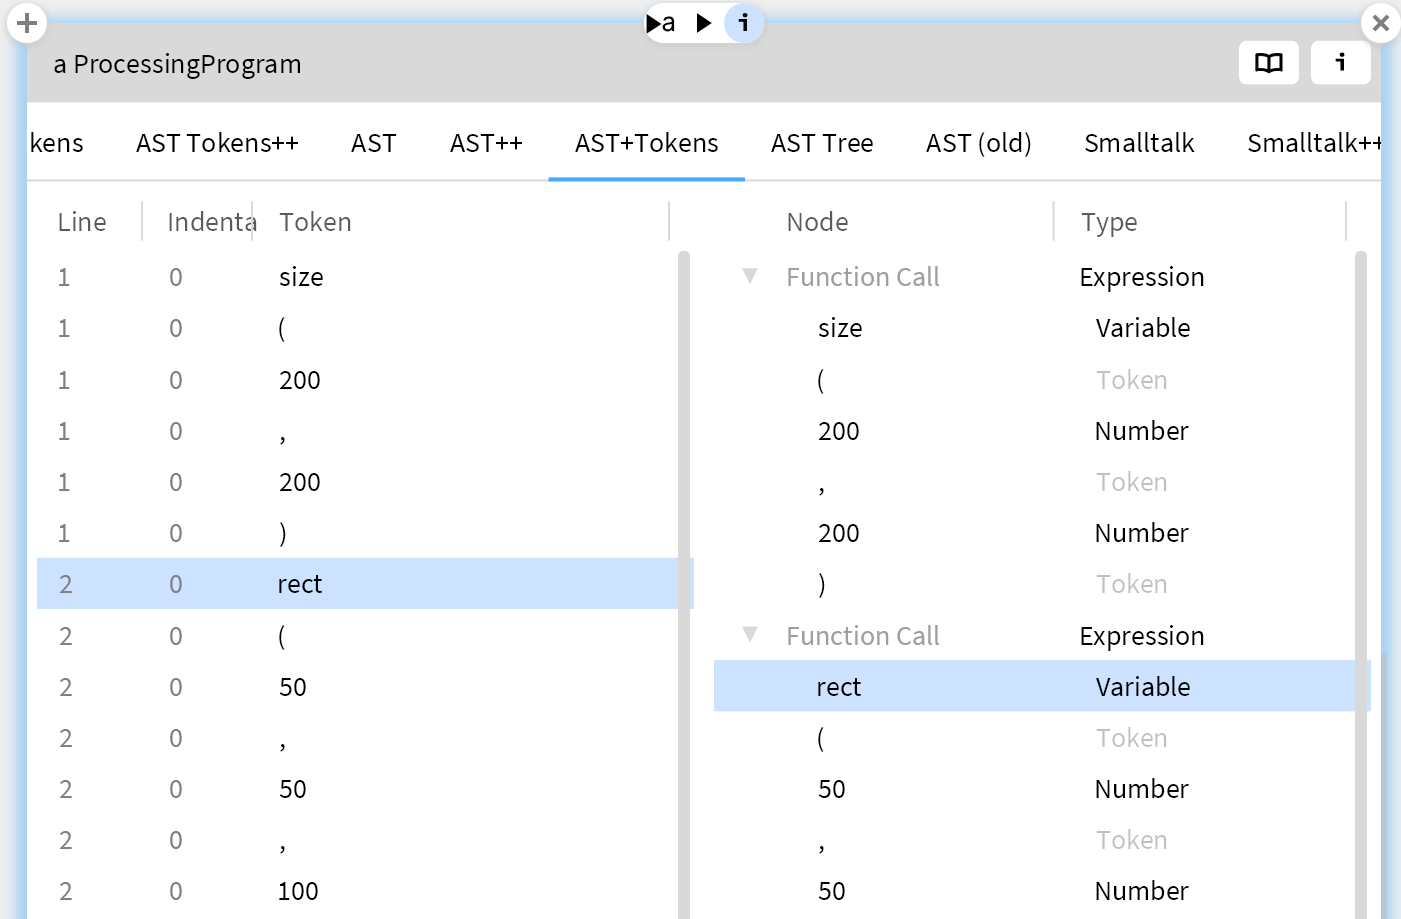
\includegraphics[width=.7\textwidth]{view_tokens_ast}
\end{cfigure}

\begin{cfigure}[fig_view_ast_tree]{The \ac{AST} as a pannable and zoomable tree}
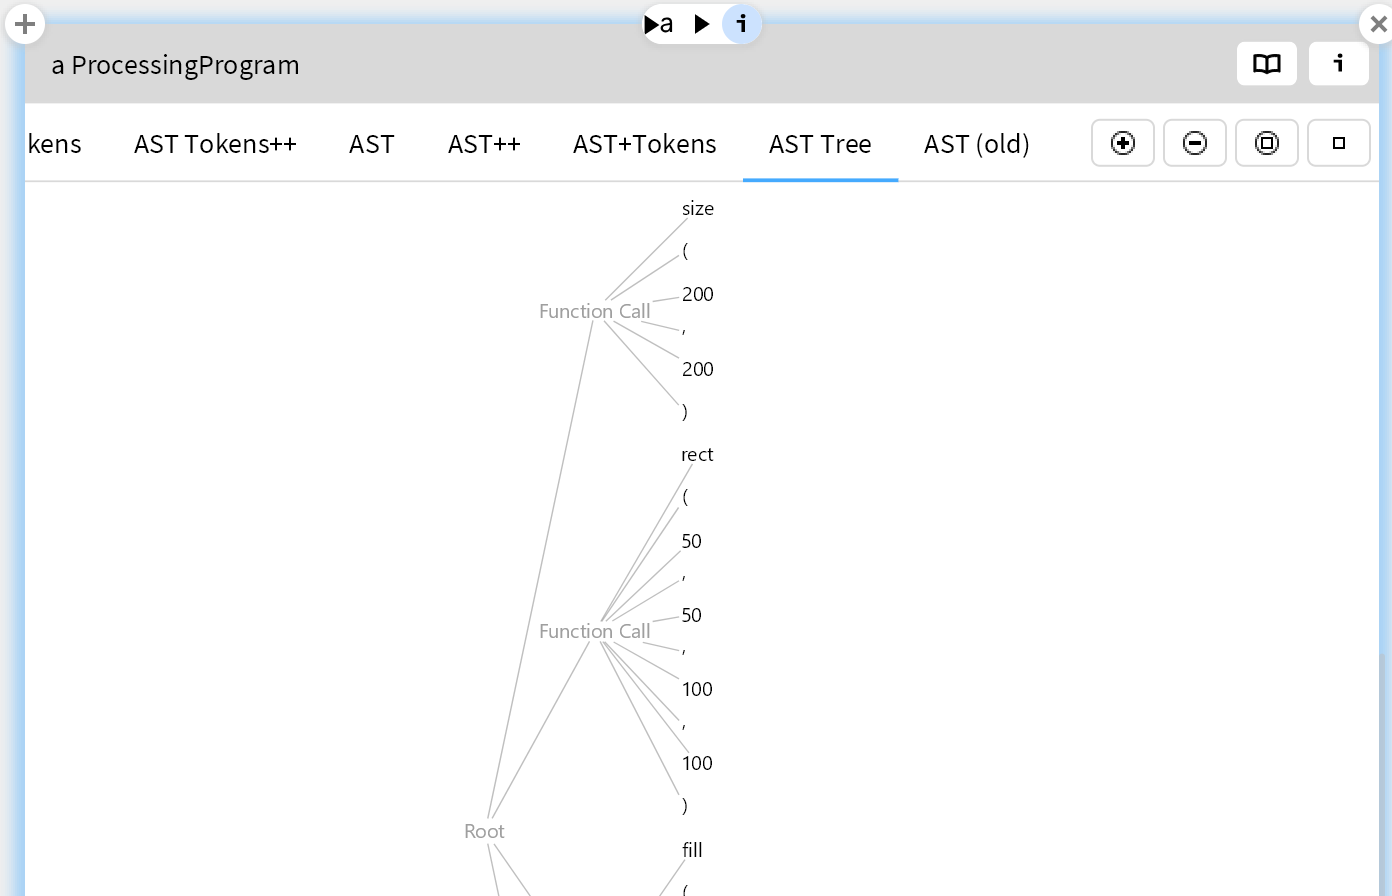
\includegraphics[width=.7\textwidth]{view_ast_tree}
\end{cfigure}

\begin{cfigure}[fig_view_transpilation]{The Transpilation view, showing Processing and Smalltalk code side by side}
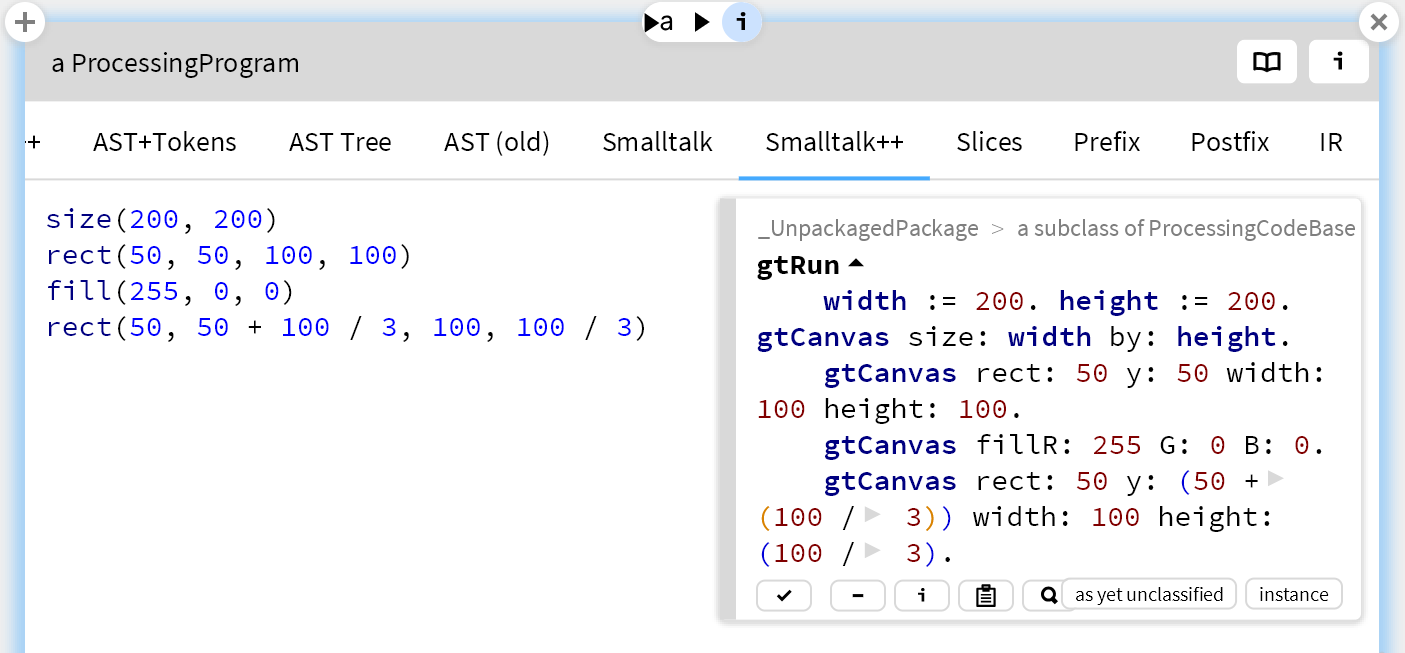
\includegraphics[width=.7\textwidth]{view_transpilation}
\end{cfigure}

\begin{cfigure}[fig_view_prefix_postfix]{Source code, \ac{AST}, and a transpilation to two pseudolanguages (with pure prefix and postfix notation)}
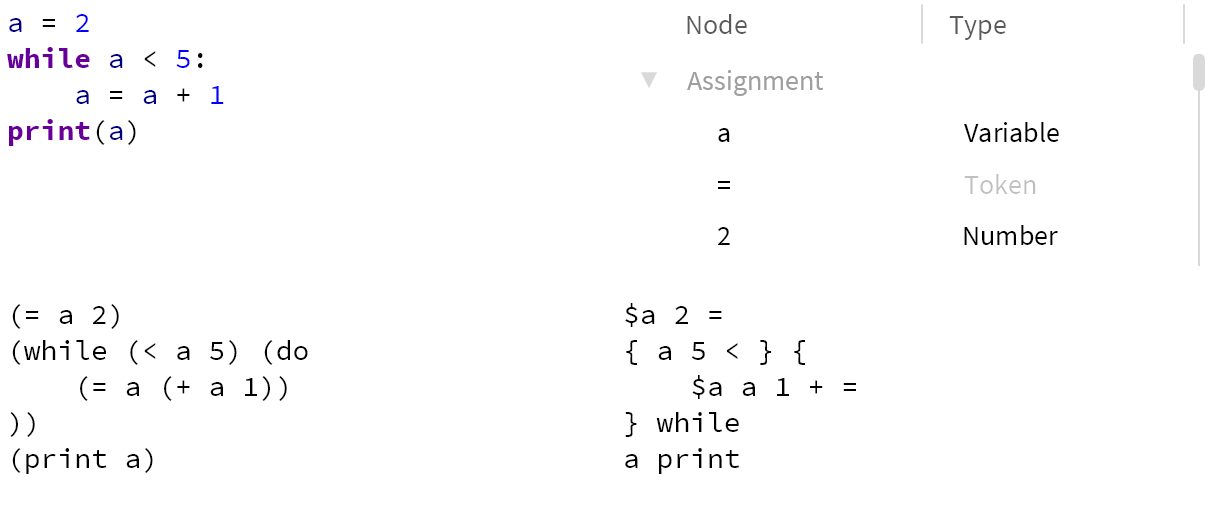
\includegraphics[width=.7\textwidth]{view_prefix_postfix}
\end{cfigure}

\begin{cfigure}[fig_view_ir_bytecode]{The \ac{IR} and Bytecode views, connected}
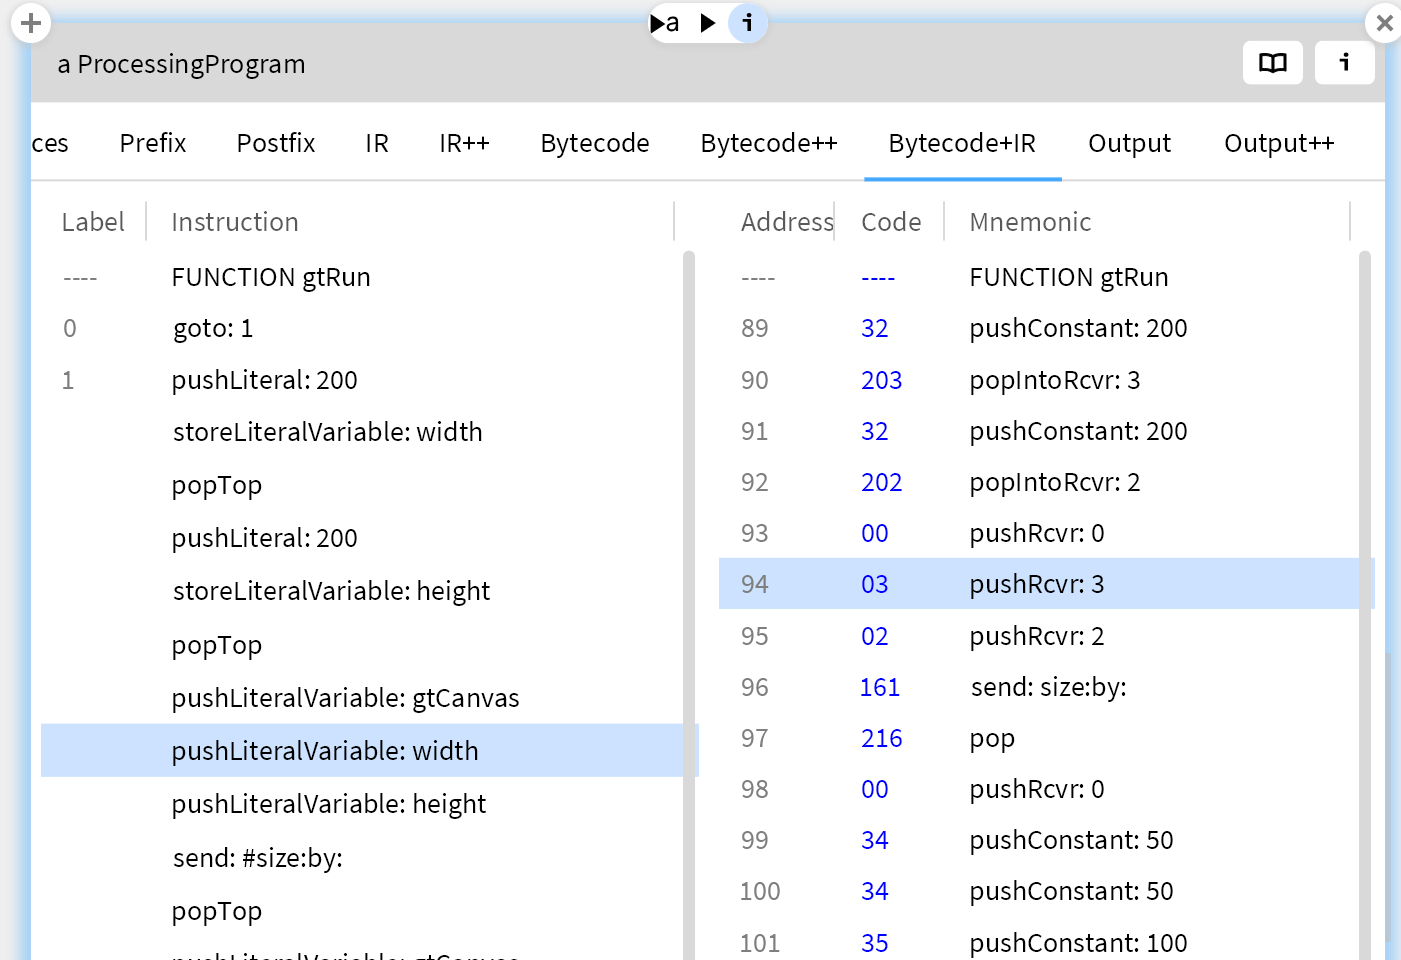
\includegraphics[width=.7\textwidth]{view_ir_bytecode}
\end{cfigure}

\begin{cfigure}[fig_view_hexdump]{The Hexdump view serializes every method into its individual bytes}
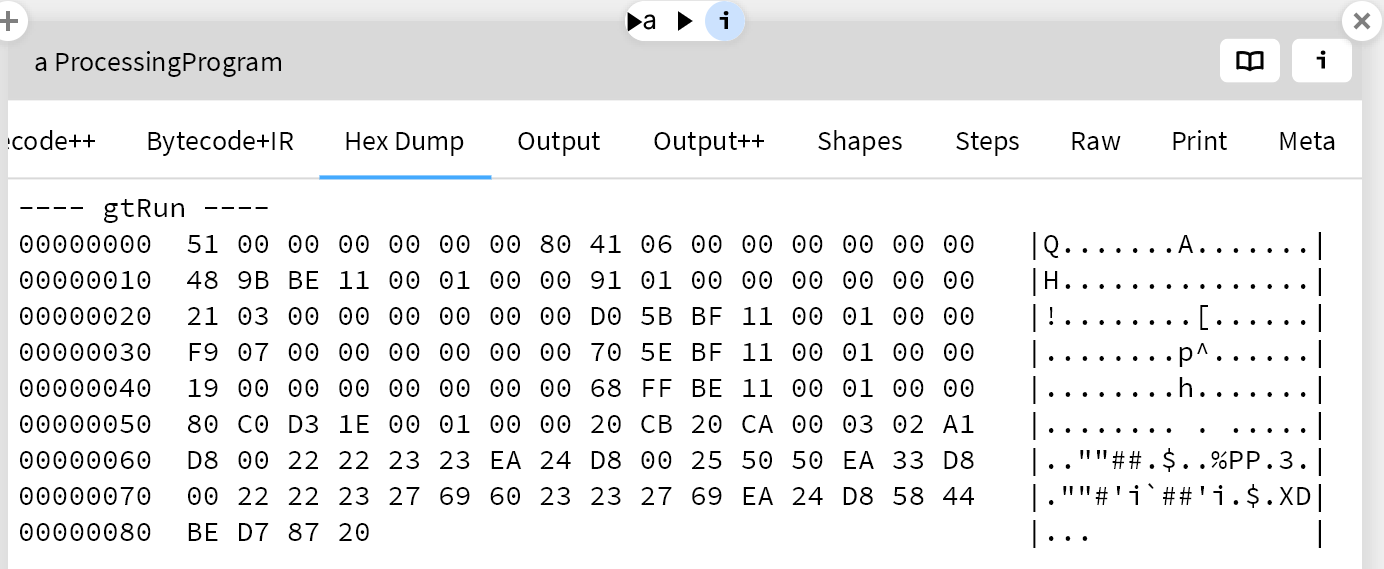
\includegraphics[width=.7\textwidth]{view_hexdump}
\end{cfigure}

\begin{cfigure}[fig_view_runsteps]{The Runsteps view allows users to step through execution and inspect variables and stack values}
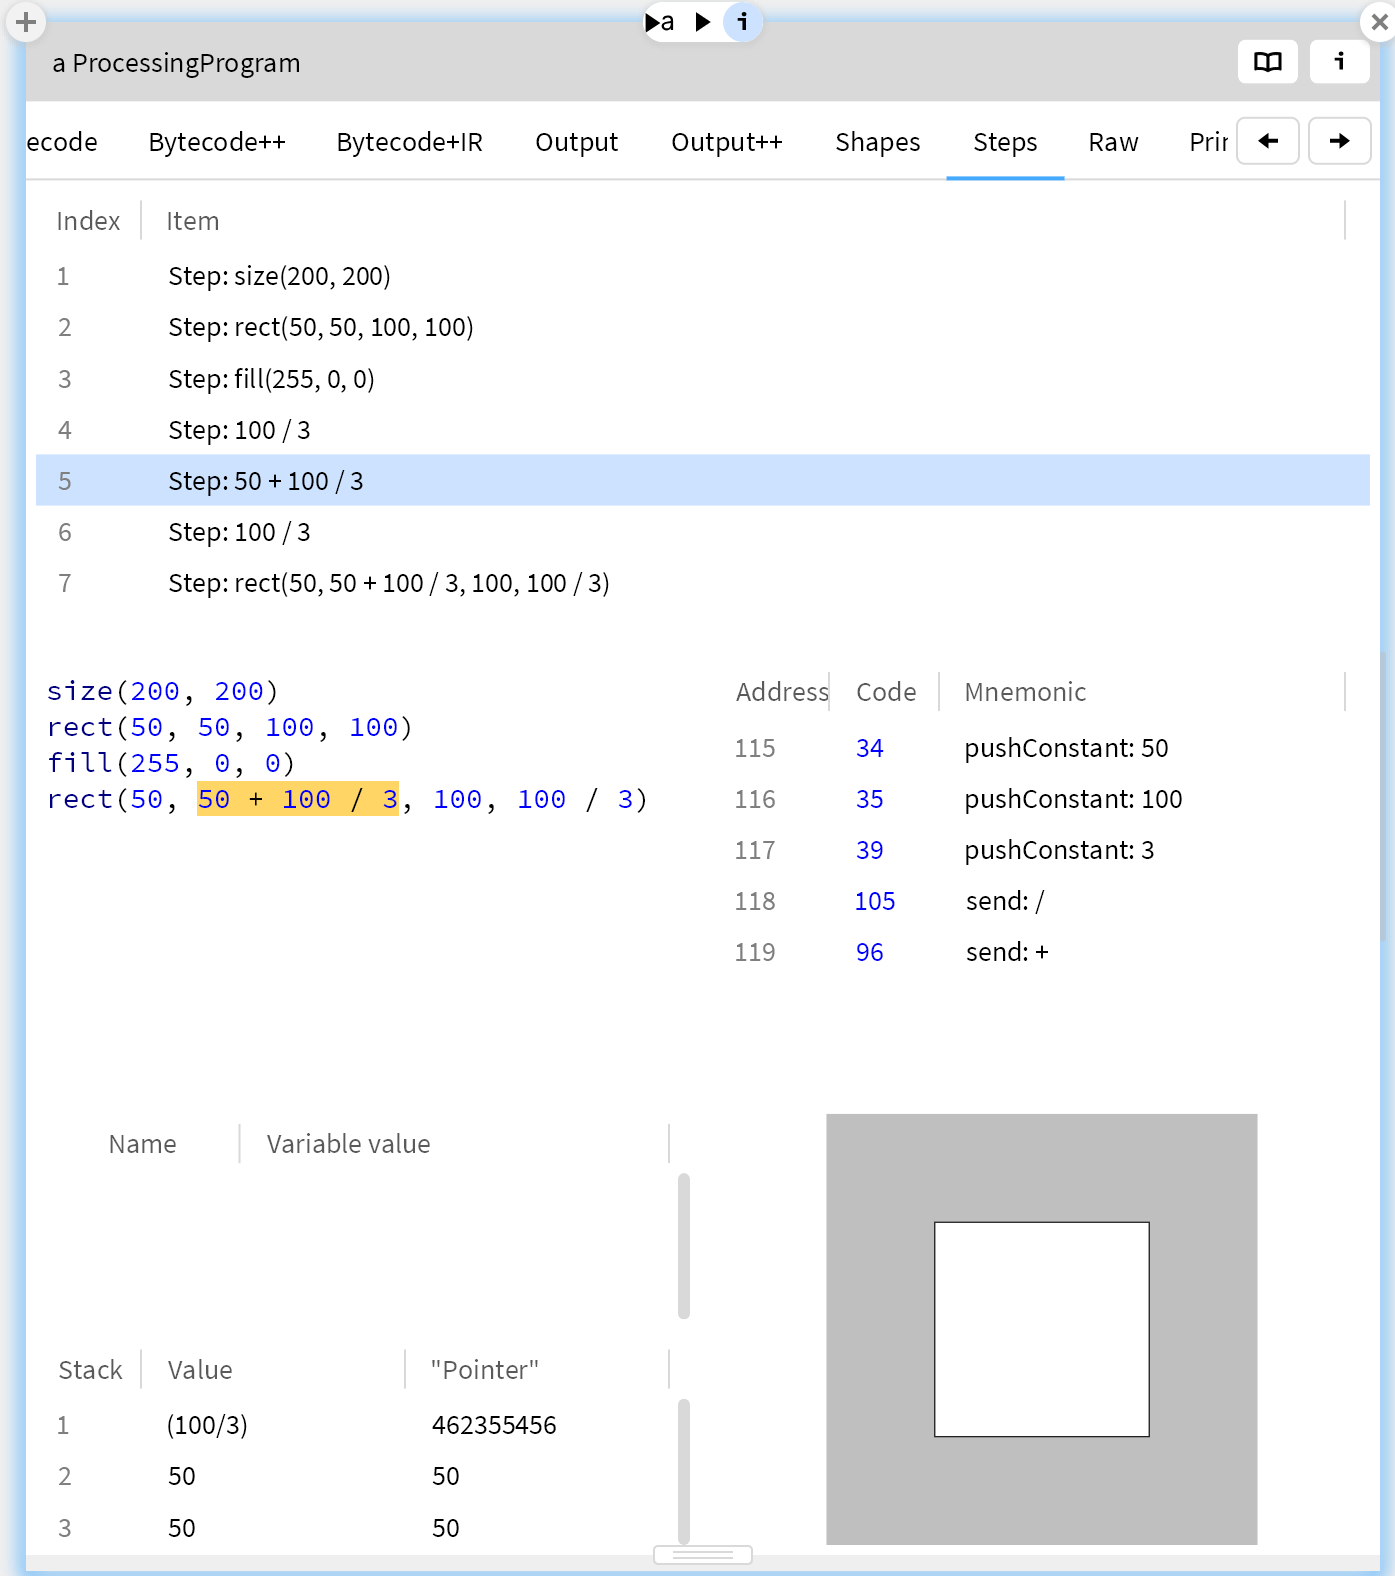
\includegraphics[width=.7\textwidth]{view_runsteps}
\end{cfigure}

\begin{cfigure}[fig_view_slices]{The Slices view shows the list of objects connecting Processing and Smalltalk code}
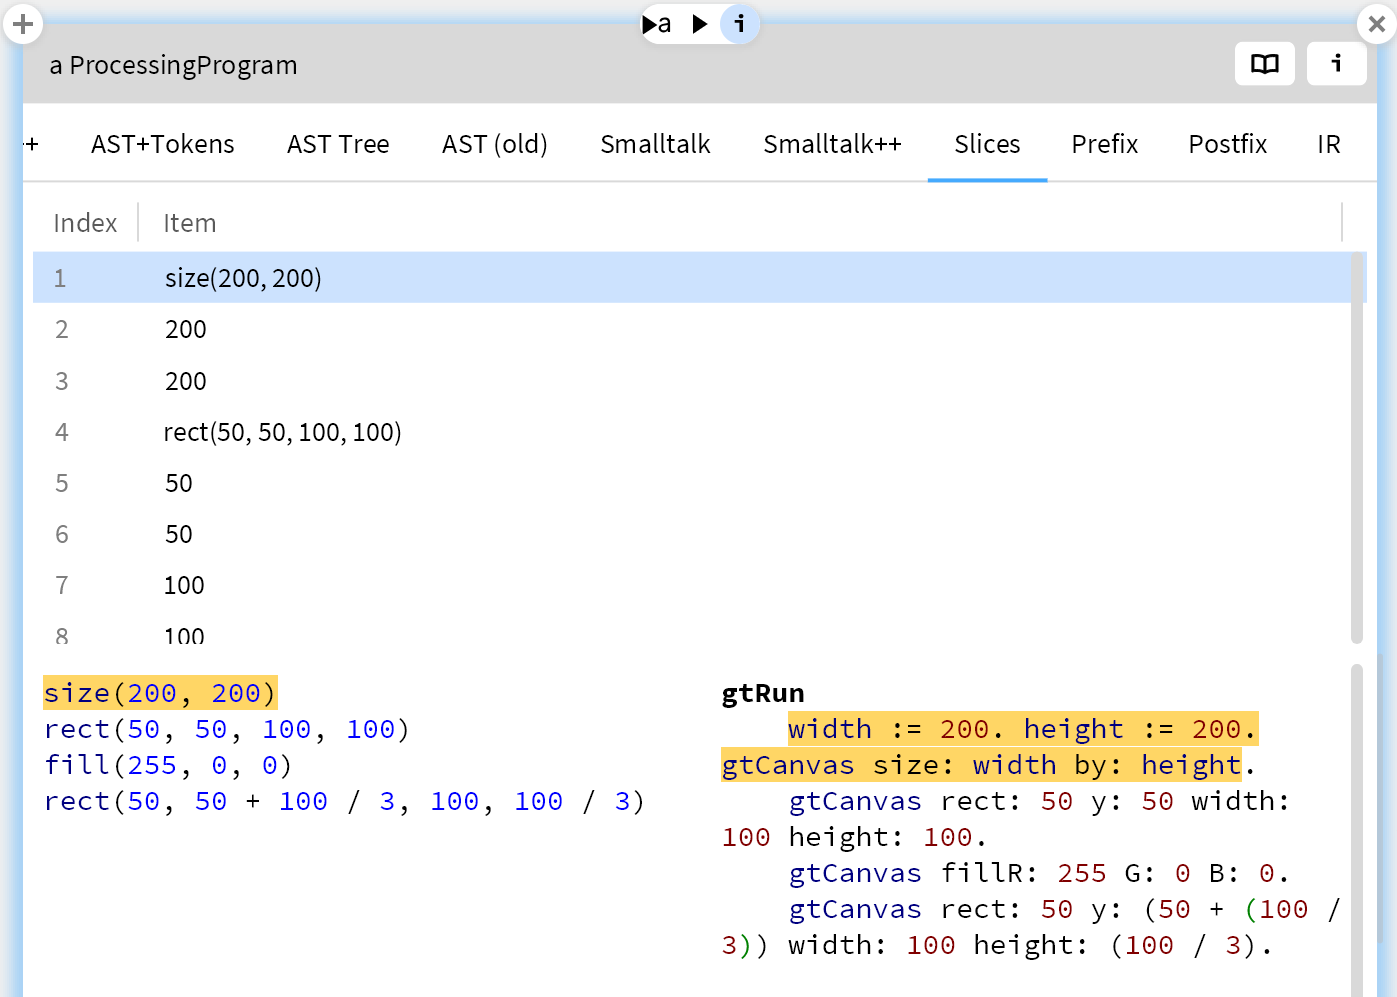
\includegraphics[width=.7\textwidth]{view_slices}
\end{cfigure}

\begin{cfigure}[fig_view_shapes]{The Shapes view displays all output shapes individually}
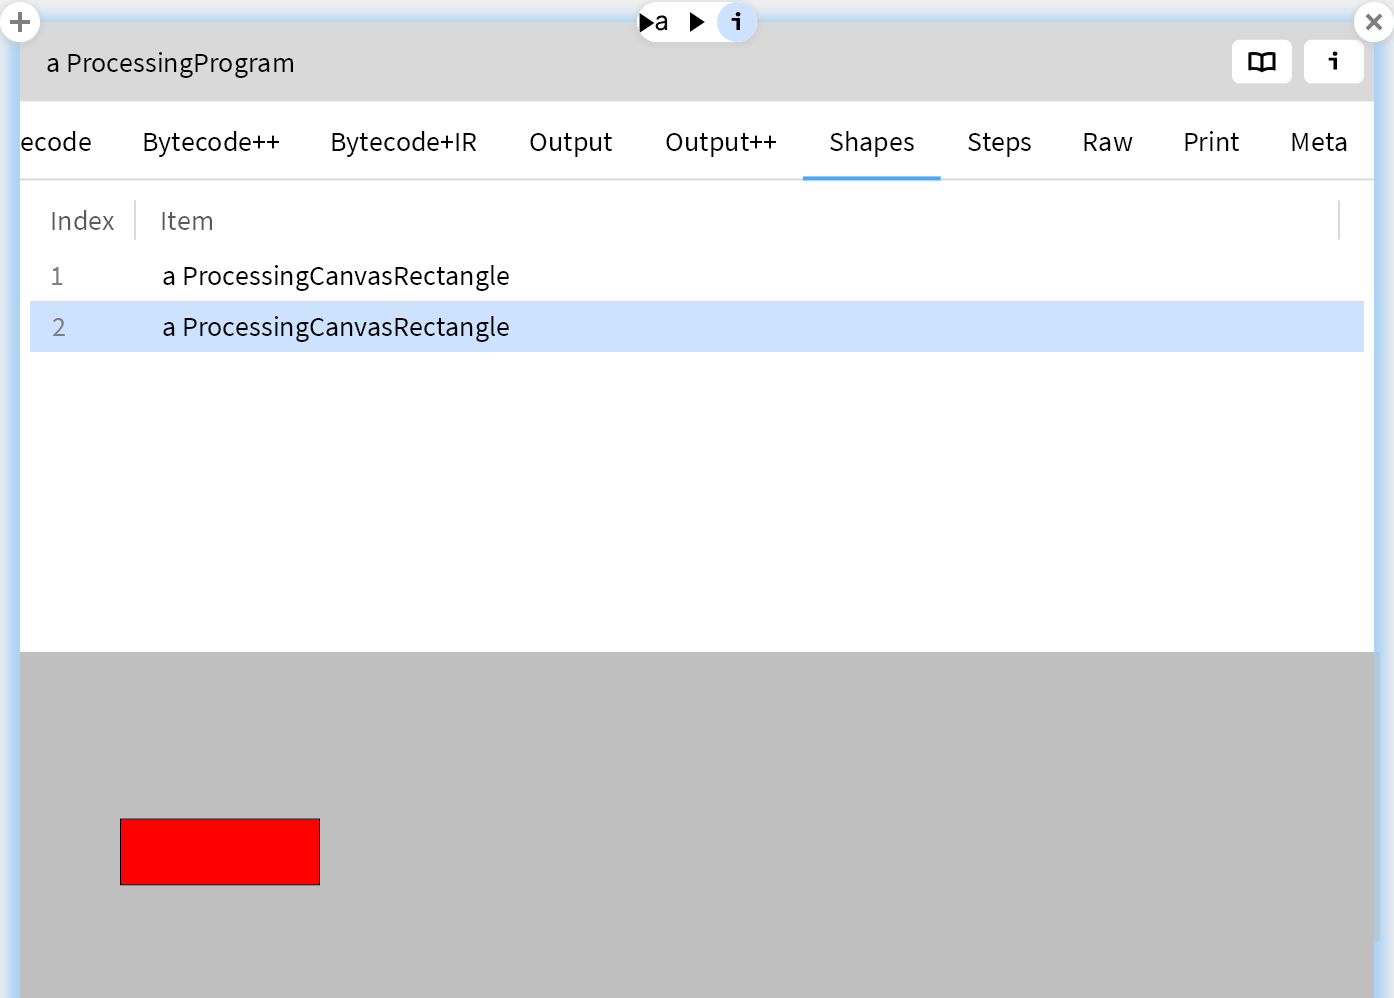
\includegraphics[width=.7\textwidth]{view_shapes}
\end{cfigure}

\begin{cfigure}[fig_view_raw]{The Raw view is provided by \ac{GT} and shows all variables of an instantiated object}
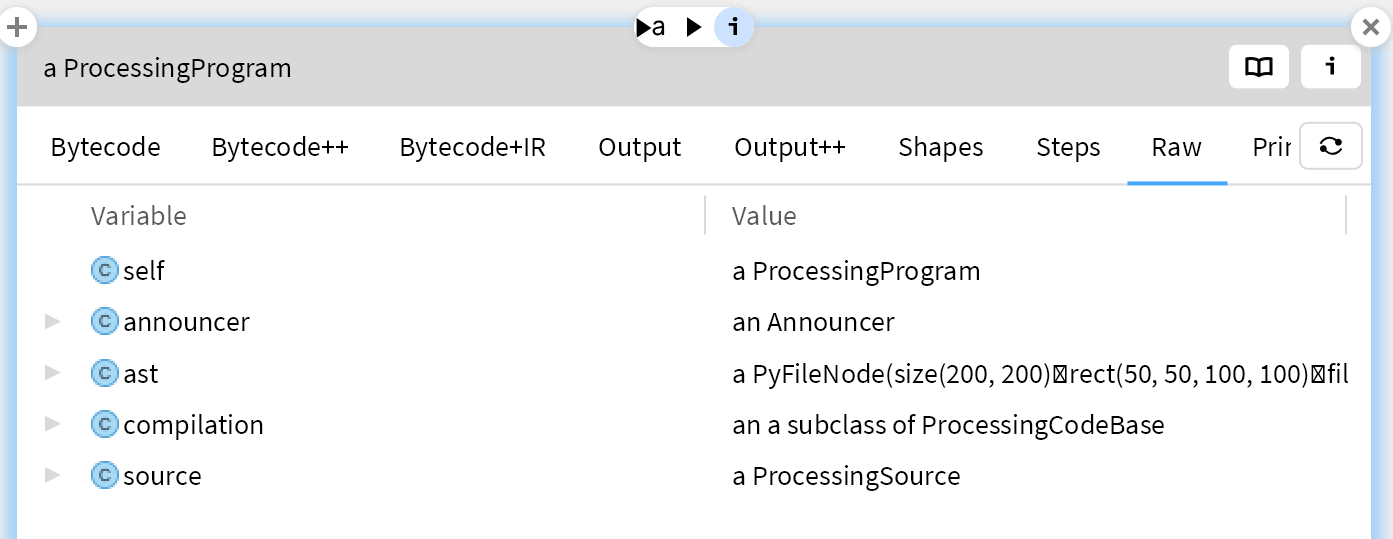
\includegraphics[width=.7\textwidth]{view_raw}
\end{cfigure}

\begin{cfigure}[fig_view_meta]{The Meta view is provided by \ac{GT} and shows all methods defined for the instantiated object}
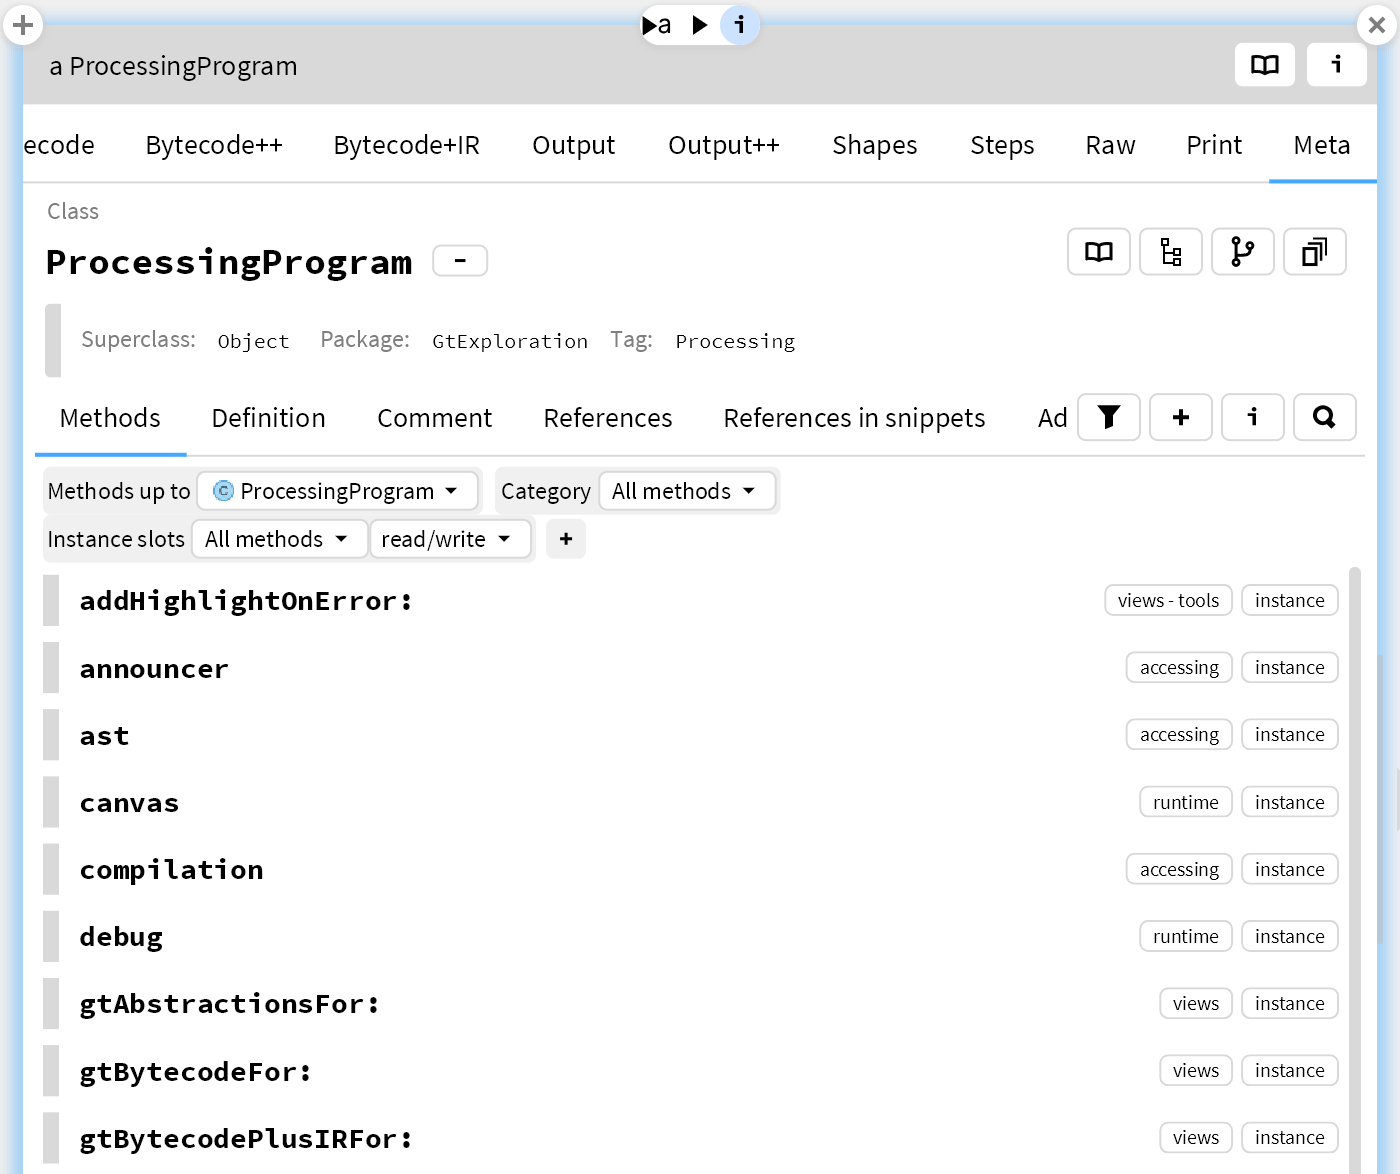
\includegraphics[width=.7\textwidth]{view_meta}
\end{cfigure}



\chapter{Questionnaires}

The questionnaires were implemented in \href{Microsoft Forms}{https://forms.office.com/} in the students' native language.


\section{Questionnaire for \ref{sc_validation_ca}} \label{app_questionnaire_1}


\subsection*{Feedback zur heutigen Unterrichtssequenz}

\begin{Questionnaire}

\item \Question{Wie hat Ihnen die heutige Unterrichtssequenz gefallen?} \\ gar nicht \Qrating{5} sehr gut

\item \Question{Welche Themen haben Sie heute alle bearbeiten k�nnen?}
\begin{Qlist}
\item Arbeiten mit Glamorous Toolkit
\item Maschinensprache und Prozessor
\item Funktionen eines Compilers
\item Anhang
\end{Qlist}

\item \Question{Wie sehr trauen Sie sich zu, die heutigen Inhalte jemand anderem zu erkl�ren?} \\ gar nicht \Qrating{5} \emph{easy-peasy}

\item \Question{Wie viele der Python-Progr�mmchen haben Sie selbst ver�ndert?}
\begin{Qlist}[$\ocircle$]
\item Keines
\item Eines
\item Zwei bis drei
\item Vier oder mehr
\end{Qlist}

\item \Question{Was ist ein Stack?} \Qlines{1}

\item \Question{Was machen Lexer und Parser?} \Qlines{1}

\item \Question{Wie gut hat die Lernumgebung f�r Sie funktioniert?} \\ gar nicht \Qrating{5} problemlos

\item \Question{Was hat Ihnen an der Lernumgebung gefallen?} \Qlines{2}

\item \Question{Welche �nderungen an der Lernumgebung w�nschen Sie sich f�r die n�chste Klasse?} \Qlines{2}

\item \Question{Wie hilfreich fanden Sie die Nebeneinanderstellungen der unterschiedlichen Schritte beim Ausf�hren/�bersetzen eines Programms?} \\ weglassen \Qrating{5} bitte mehr davon

\item \Question{Beschreiben Sie in eigenen Worten: Wie wird ein Programm auf einem Prozessor ausgef�hrt?} \Qlines{2}

\item \Question{Beschreiben Sie in eigenen Worten: Wie wird ein Programm in einer Hochsprache wie Processing f�r den Prozessor aufbereitet?} \Qlines{2}

\item \Question{Was hatte das heutige Thema mit Silizium, Transistoren, Gattern und Schaltungen zu tun?} \Qlines{2}

\suspend{Questionnaire}


\subsection*{Feedback zum Informatikunterricht der letzten zwei Jahre}

\resume{Questionnaire}

\item \Question{Was war f�r Sie das Highlight vom Informatik-Unterricht? (Was hat Ihnen am meisten Eindruck gemacht?)} \Qlines{1}

\item \Question{Was ist Ihnen vom Informatik-Unterricht alles geblieben (einige Stichworte zum Stoff)?} \Qlines{2}

\item \Question{Was hat Ihnen am Informatik-Unterricht gefallen?} \Qlines{2}

\item \Question{Wenn Sie mir vor zwei Jahren einen Hinweis geben k�nnten: Was h�tten Sie sich f�r den Unterricht anders gew�nscht?} \Qlines{2}

\end{Questionnaire}



\section{Questionnaire for \ref{sc_validation_compiler}} \label{app_questionnaire_2}


\subsection*{Feedback zur heutigen Unterrichtssequenz}

\begin{Questionnaire}

\item \Question{Wie hat Ihnen die heutige Unterrichtssequenz gefallen?} \\ gar nicht \Qrating{5} sehr gut

\item \Question{Welche Themen haben Sie heute alle bearbeiten k�nnen?}
\begin{Qlist}
\item Arbeiten mit Glamorous Toolkit
\item Human Resource Machine (aus Maschinensprache und Prozessor)
\item Lexer und Parser
\item Transpiler und Compiler
\item Optimierer
\end{Qlist}

\item \Question{Wie sehr trauen Sie sich zu, die heutigen Inhalte jemand anderem zu erkl�ren?} \\ gar nicht \Qrating{5} \emph{easy-peasy}

\item \Question{Wie viele der Python-Progr�mmchen haben Sie selbst ver�ndert?}
\begin{Qlist}[$\ocircle$]
\item Keines
\item Eines
\item Zwei bis drei
\item Vier oder mehr
\end{Qlist}

\item \Question{Weshalb kann ein Prozessor ein Processing-Programm nicht ohne �bersetzung ausf�hren} \Qlines{1}

\item \Question{Was machen Lexer und Parser?} \Qlines{1}

\item \Question{Wie gut hat die Lernumgebung f�r Sie funktioniert?} \\ gar nicht \Qrating{5} problemlos

\item \Question{Was hat Ihnen an der Lernumgebung gefallen?} \Qlines{2}

\item \Question{Welche �nderungen an der Lernumgebung w�nschen Sie sich f�r die n�chste Klasse?} \Qlines{2}

\item \Question{Wie hilfreich fanden Sie die Nebeneinanderstellungen der unterschiedlichen Schritte beim Ausf�hren/�bersetzen eines Programms?} \\ weglassen \Qrating{5} bitte mehr davon

\item \Question{Beschreiben Sie in eigenen Worten: Wie wird ein Programm in einer Hochsprache wie Processing f�r den Prozessor aufbereitet?} \Qlines{2}

\item \Question{Was hatte das heutige Thema mit Codierung und was mit Programmieren zu tun?} \Qlines{2}

\suspend{Questionnaire}


\subsection*{Feedback zum Informatikunterricht}

\resume{Questionnaire}

\item \Question{Was war f�r Sie das Highlight vom Informatik-Unterricht? (Was hat Ihnen am meisten Eindruck gemacht?)} \Qlines{1}

\item \Question{Was ist Ihnen vom Informatik-Unterricht alles geblieben (einige Stichworte zum Stoff)?} \Qlines{2}

\item \Question{Was hat Ihnen am Informatik-Unterricht gefallen?} \Qlines{2}

\item \Question{Welche �nderungen w�nschen Sie sich f�rs kommende Schuljahr in Informatik?} \Qlines{2}

\end{Questionnaire}
